\chapter{Multifactorial emotion estimation}
\label{ch:literature-multifactorial}

Previous chapters demonstrate the use of physiological signals and facial information applied separately to emotion estimation. The use of a single signal for the assessment is feasible, however a mapping process based on a multifactorial analysis, when more than one signal is used, is more likely to produce accurate results \parencite{kukolja2014comparative}. A combination of signals can reduce the interference/noise caused by signal manipulation.

Physiological signals, e.g. HR, are considered reliable sources since they are hard to fake (because of their link to the ANS), differently from facial expressions \parencite{Landowska}, for instance. When combined in the same analysis, however, those signals can complement each other and provide more information about emotional states.

The following sections present works related to multifacotiral emotion estimation categorized by contact (use of physical sensors) and non-contact (remote analysis) approaches.

\section{Approaches based on physical contact and sensors}

The first multifactorial analysis approaches were based on obtrusive measurements of the input signals, where physical sensors were used. \textcite{Chanel_2011}, for instance, demonstrate the use of multifactorial input analysis to measure emotions and involvement in a game context. Participants play Tetris in different difficulty conditions while being monitored by a variety of sensors, which include a respiration belt and an electroencephalogram (EEG) system. The data from the EEG and the other peripheral signals are computed into two groups of features, which are used to train classifiers to recognize the states: boredom (low pleasure and low pressure, associated with easy difficulty), engagement (higher pleasure and motivation, associated with medium difficulty) and stress (anxiety and low pleasure, associated with hard difficulty). The classification accuracy of the model varies between 48\% and 55\% for different input signals, classifiers and feature selection.

\textcite{grundlehner2009design} also use physical sensors to perform real-time continuous arousal monitoring. The authors record and use four signals from subjects to estimate arousal: electrocardiogram (ECG), respiration, skin conductance and skin temperature. The ECG is used to calculate HRV, which is then used in the estimation. The data used for emotion-triggering is based on videos, sounds and a cognitive demanding game. A regression analysis is performed to identify the importance of the features in the estimation of arousal. $HRV_{LF}$ and $HRV_{HF}$ are not significant when compared to the other signals (e.g. skin conductance), while the standard deviation of HRV presents a significant weight. The arousal prediction matches the hypothesized arousal events marked by the authors in each of the emotion-triggering content. The results, however, were performed with controlled, pre-defined events that are expected to cause reactions, which might be related to arousal. More subtle or dynamic interactions, such as the ones obtained when a subject plays a digital game, might not be identified or detected by the approach proposed by the authors.

\textcite{bailenson2008real} use a combination of physiological signals (obtained from physical sensors) and facial expressions. The authors use a machine learning model to map the input signals to emotions (sadness or amusement). The training data used for the machine learning model is based on recordings of participants while they watched a video containing different emotion-triggering segments (neutral, amusement and sadness). Additionally 15 physiological signals are also used, among them HR, skin conductance level and finger temperature. The video recordings are annotated by professional coders. The annotated video frames are used in conjunction with the physiological signals to produce the predicting model. The authors compare the performance of models built from different data sources, such as the data from all subjects (general model), or from the female/male population (gender-specific model) or from a single individual (person-specific model). The model performs better when categorizing emotions instead of predicting its intensities and when detecting amusement instead of sadness. Additionally the person-specific model outperforms the other two variations, suggesting that a person-tailored model might be more effective in identifying features (even the more subtle ones) than a general-purpose model. The results also state that a model built from a combination of facial and physiological information is more efficient than a model built with either one alone.

\begin{figure}
\centering
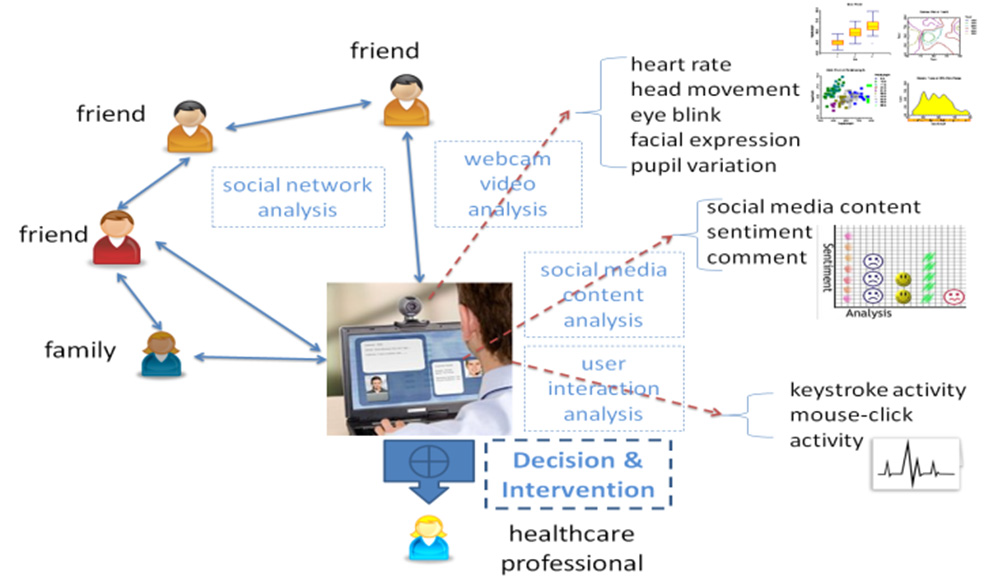
\includegraphics[width=0.9\linewidth]{Content/figures/zhou.png}
\caption{Non-obtrusive and remote approach based on multifactorial analysis to identify user emotion. Reproduced from \textcite{mental}.}
\label{fig:zhou}
\end{figure}

\section{Approaches based on remote, non-contact analysis}

\textcite{mental} propose a completely non-obtrusive and remote approach based on multifactorial analysis to identify user emotion, as illustrated in Figure \ref{fig:zhou}. The main goal of such approach is aimed at monitoring patients mental health states. The model was created by weighting different features created from input signals, all obtained unobtrusively from a video of the subject's face and the textual content he/she created during the session (e.g. a reply to a tweet). The features are physiological (HR and pupil radius), physical (head movement rate, facial expression, eye blinking rate), based on human-computer interactions (mouse and keyboard usage rate) and based on sentiment analysis of social content (images and textual tweets). All features are used to train a multi-class classifier (based on logistic regression), which learns about the three possible emotion states: negative, neutral and positive. The emotion inference is performed in real-time and based on a probability rule: the state suggested by the classifier with the highest intensity is assumed to be the current subject's emotional state. The results show an accuracy rate of 89\% for negative, 56\% for neutral and 78\% for positive state identification. The authors do not specify, however, how much each input signals contributes to the emotional output. Additionally it is not possible to infer if such approach could be used outside the controlled environment created by the authors, which requires a simulation of a social network filled with previously defined and known content in order to work.

\textcite{mcduff2014remote} also use a camera to remotely measure cognitive stress via HRV. Participants are recorded while resting and while silently performing a mental arithmetic task. Facial landmarks are automatically detected and a ROI containing part of the subject's face is selected for analysis. Using a spacial average of the pixel intensities in each frame, a PPG signal is calculated through independent component analysis (ICA) and blood volume pulse (BVP) is extracted. Based on the discovered BVP, several other physiological parameters are calculated, such as HR, respiratory rate (RR), $HRV_{LF}$ and $HRV_{HF}$. The remote measurement of all physiological signals is in agreement with a physical device used as ground truth. Using those parameters, the authors construct a classifier, modeled with Naive Bayes and support vector machine (SVM), for predicting whether the subject is under cognitive stress. The input features used for the models are mean heart rate, mean respiratory rate, normalized $HRV_{LF}$ power, normalized $HRV_{HF}$ power and $HRV_{LF/HF}$ power ratio for each session. Results show that the prediction accuracy is 85\% using SVM, demonstrating that the input signals are sensitive enough to measure the cognitive stress state. The HRV components and the RR are the strongest predictors, while the is was not significantly different between the two detectable states. \textcite{mcduffcogcam} perform further investigations, however using different cognitive tasks (two cognitive demanding games). A person-independent machine learning model based on HR, HRV, $HRV_{LF}$, $HRV_{HF}$ (along with normalized and combined versions of those signals) and breathing rate is used to classify the stress level of the subjects. According to the authors, the average heart rate and breathing rate are not significantly different in any case, which differs from previous findings of other authors. The variations of $HRV_{LF}$ and $HRV_{HF}$, however, are significantly different during the cognitive tasks compared to the rest period; higher $HRV_{LF}$ and lower $HRV_{HF}$ power are found in both cognitive tasks compared to the rest period, which aligns with findings of previous work. Authors also point out that the stress predictions made by the model are consistent with the self-reported answers. The two participants with the highest self-reported stress level show the highest predicted stress level, while the two participants with the lowest self-reported stress level also present the lowest predictions. %It emphasizes the challenges associated with the great variability between individuals regarding physiological signals and emotional state, such as stress.

\begin{figure}[h]
    \centering
    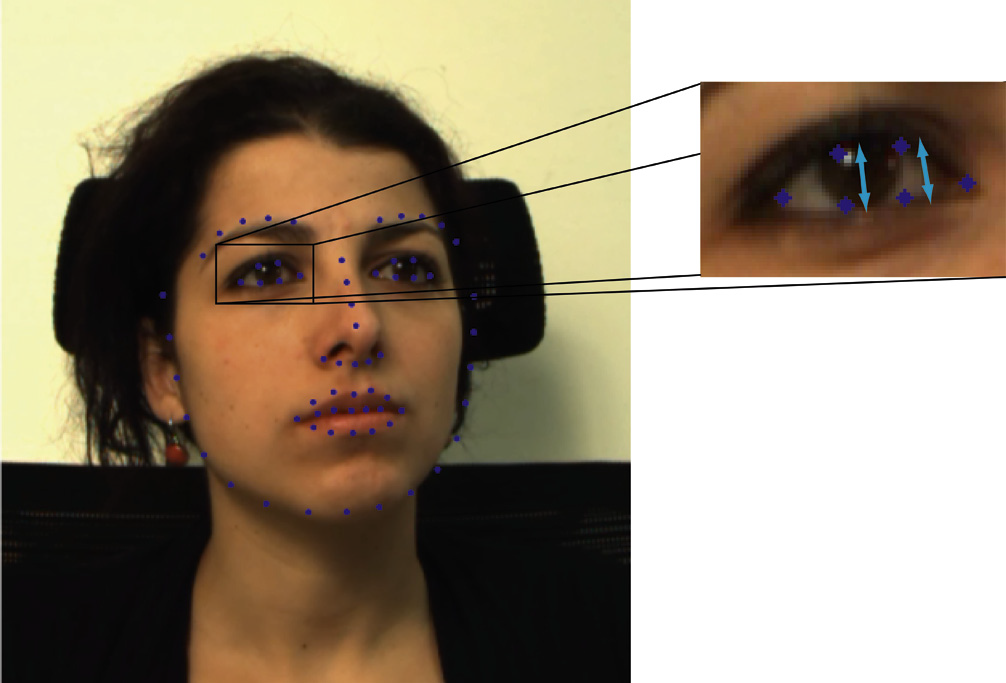
\includegraphics[width=0.7\linewidth]{Content/figures/giannakakis2017stress-eye.png}
    \caption{Highlight of distance calculation regarding eye aperture. Reproduced from \textcite{giannakakis2017stress}.}
    \label{fig:giannakakis2017stress-eye}
\end{figure}

Finally \textcite{giannakakis2017stress} present an approach for detection of stress/anxiety based on eye blink, mouth/head movements and HR estimations using rPPG. Participants are recorded while performing a set of tasks designed to trigger emotional responses, such as talking in a foreign language, remembering a sad incident, visualizing images/videos and playing a gamified cognitive test, i.e. Stroop test. Facial cues are obtained from an automatically detected ROI. Those cues are used to extract facial features, which are related to eyes, mouth, and head movement. Figure \ref{fig:giannakakis2017stress-eye} highlights the facial analysis used in the calculation of eye apperture, which is one of the features extracted and used in the emotion detection. The extracted features, including HR information estimated using rPPG, are selected and ranked accordinly to maximize a machine learning classification step. Different classifiers are employed, which yield different classification accuracy rates. For each task performed by the subjects, classification accuracy ranges between 80\% and 90\% taking into account the most efficient classifier. It is noted by the authors that the observation of stressful images and the interaction with the Stroop test appear to be the most consistent across the classifiers employed.
